% !Mode:: "TeX:UTF-8"

\chapter{结果展示}
\label{ch:results}

本章将选择DODT在KITTI追踪数据集上的一些结果进行展示,以便读者能够更好的了解DODT的性能。

\section{验证集结果展示}
\label{val_results}
本小节我们可视化了三对模型在KITTI目标追踪验证数据集上的预测结果。这三对模型分别是AVOD与DODT(T=3) 、 DODT(T=1)与DODT(T=3) 以及Based\_DODT 与 DODT(T=3),分别对应了图\ref{fig:avod_dodt}、图\ref{fig:dodt_1_3}以及图\ref{fig:dodt_based}。所有选取的可视化帧都是步长为3的连续关键帧,图中绿色框为KITTI官方提供的标签框,蓝色为我们新添加的标签框。图\ref{fig:avod_dodt}可视化的是第20段视频的第18、21和24帧,可以看出相比于AVOD,DODT(T=3) 对远处目标以及新添加标签的目标预测更好。图\ref{fig:dodt_1_3}可视化的是第18段视频的第150、153和156帧,可以看出大步长有利于轨迹的延伸,从而使得模型对远处物体预测性能更好。图\ref{fig:dodt_based}可视化的是第20段视频的第30、33和36帧,可以看出时序信息以及MoI插值算法有利于保持目标状态的长程联系性。


\begin{figure}[t]
	\centering
	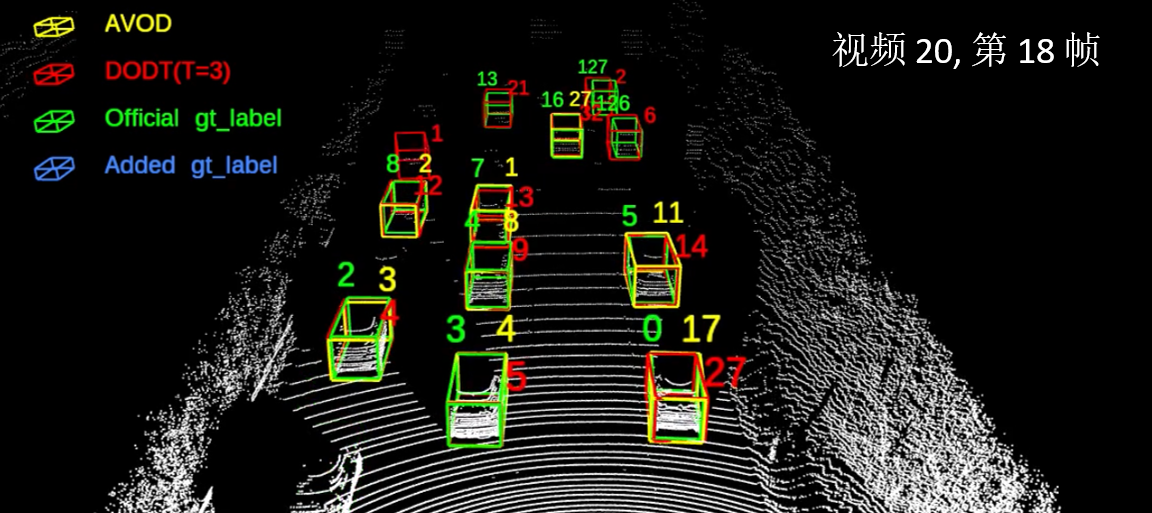
\includegraphics[width=\textwidth]{./imgs/viz_results/val/avod_dodt_01.png}\vspace{1pt}
	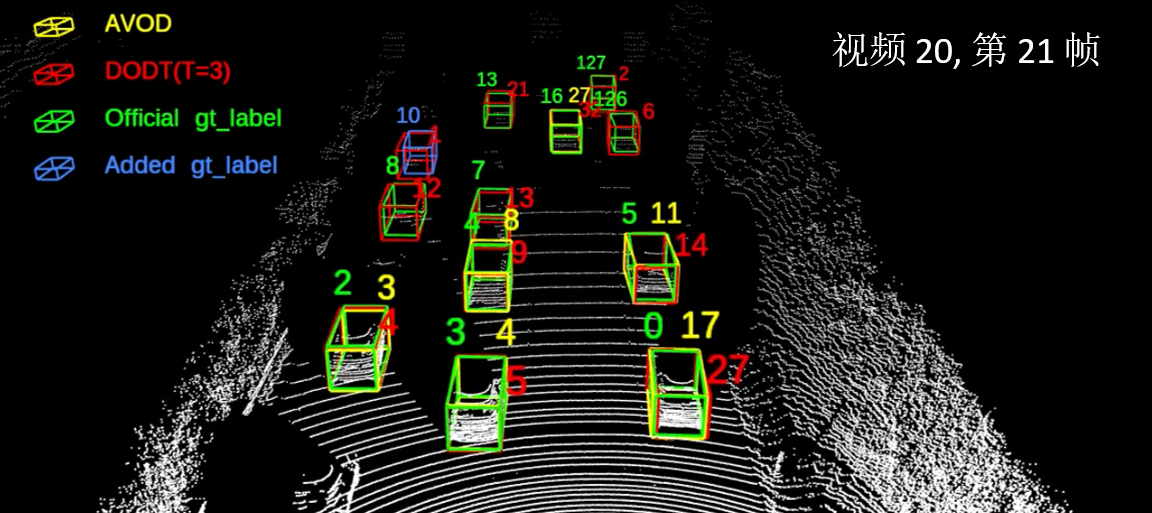
\includegraphics[width=\textwidth]{./imgs/viz_results/val/avod_dodt_02.png}\vspace{1pt}
	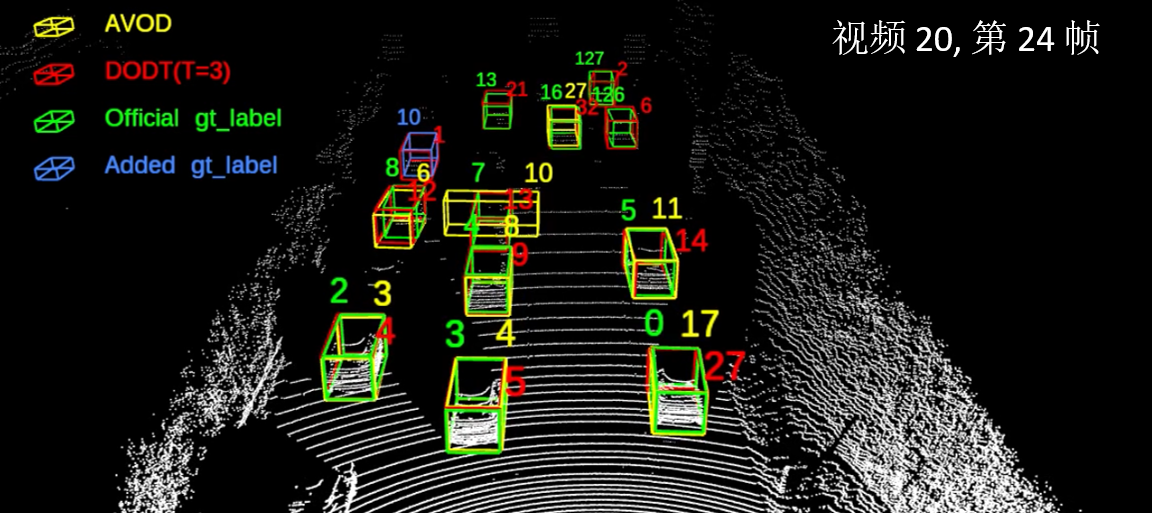
\includegraphics[width=\textwidth]{./imgs/viz_results/val/avod_dodt_03.png}
	\caption{AVOD与DODT($\tau=3$)对比结果。}
	\label{fig:avod_dodt}
\end{figure}

\begin{figure}[t]
	\centering
	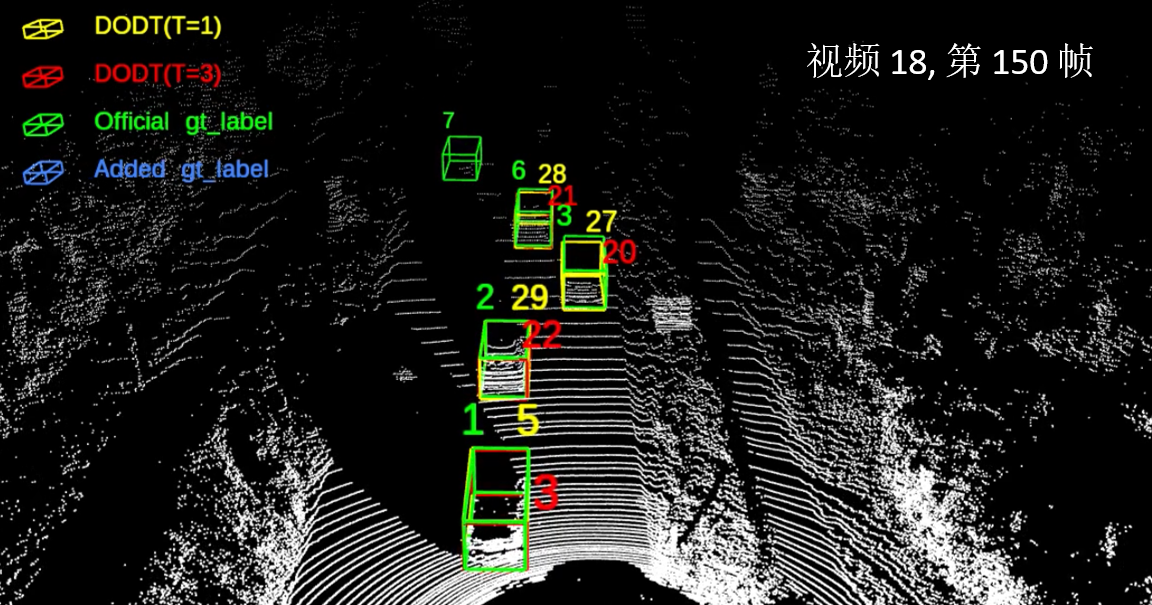
\includegraphics[width=\textwidth]{./imgs/viz_results/val/dodt_1_3_01.png}\vspace{1pt}
	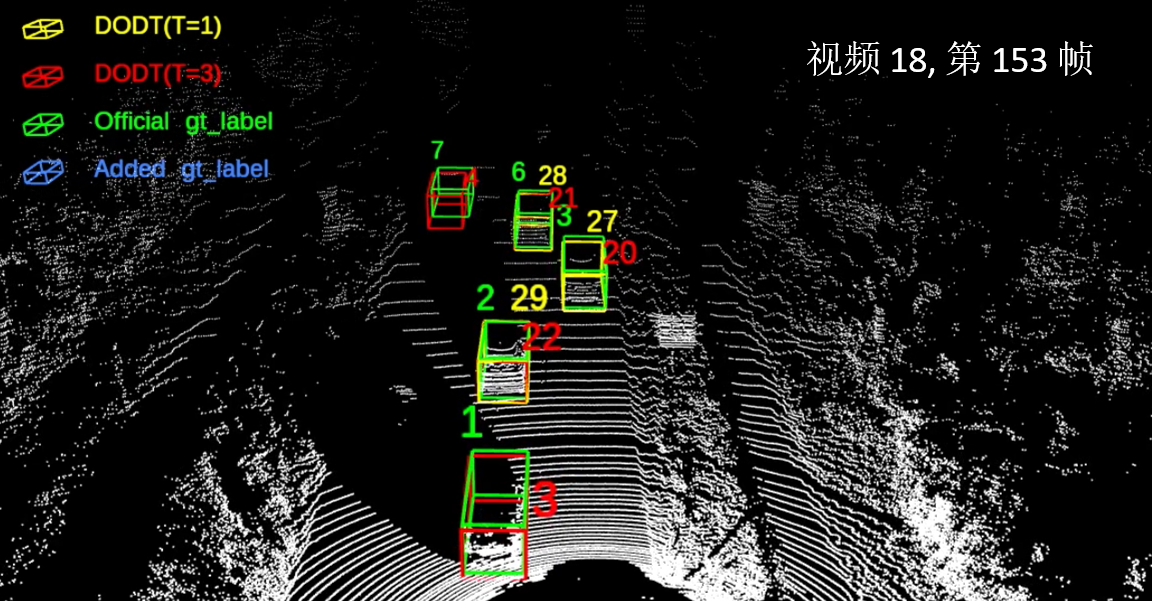
\includegraphics[width=\textwidth]{./imgs/viz_results/val/dodt_1_3_02.png}\vspace{1pt}
	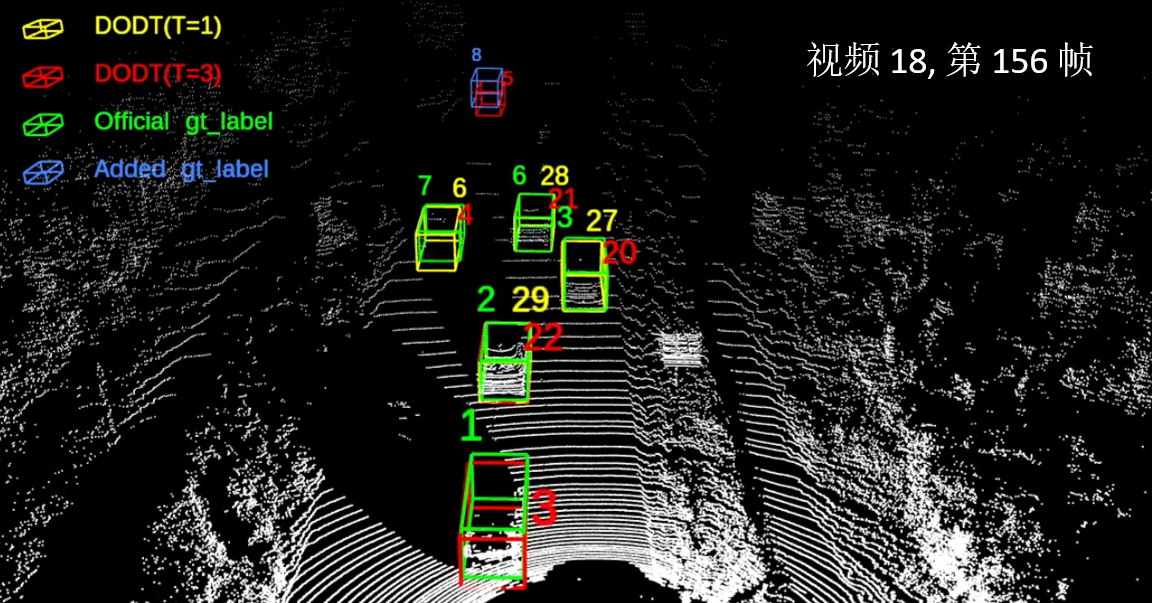
\includegraphics[width=\textwidth]{./imgs/viz_results/val/dodt_1_3_03.png}
	\caption{DODT($\tau=1$)与DODT($\tau=3$)对比结果。}
	\label{fig:dodt_1_3}
\end{figure}

\begin{figure}[t]
	\centering
	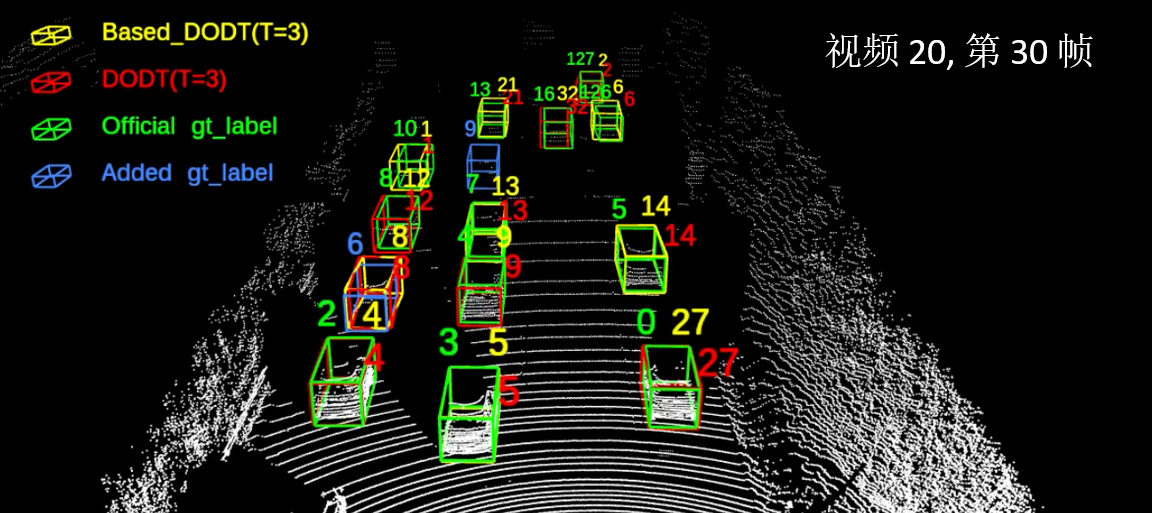
\includegraphics[width=\textwidth]{./imgs/viz_results/val/dodt_based_01.png}\vspace{1pt}
	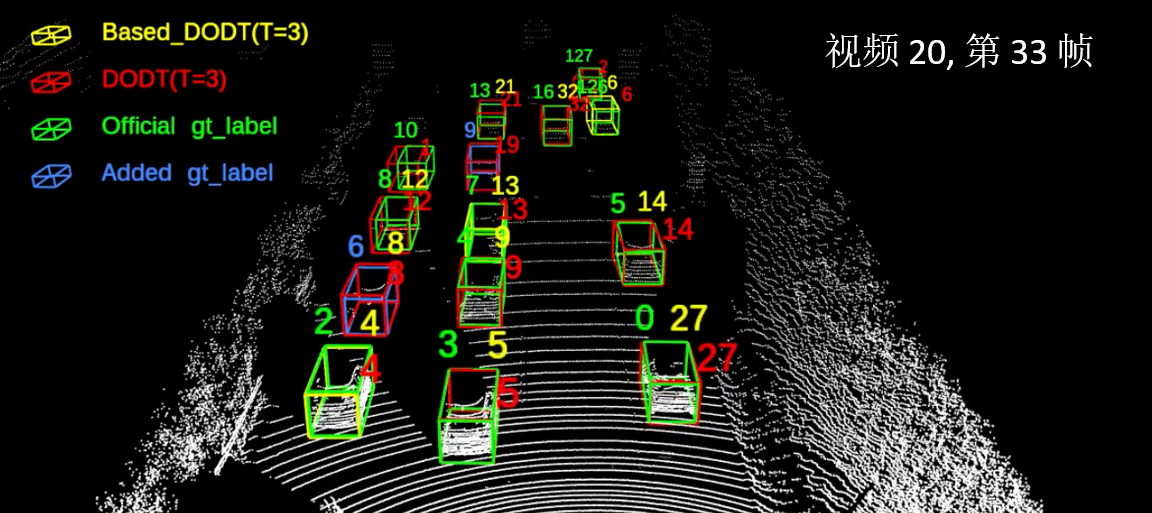
\includegraphics[width=\textwidth]{./imgs/viz_results/val/dodt_based_02.png}\vspace{1pt}
	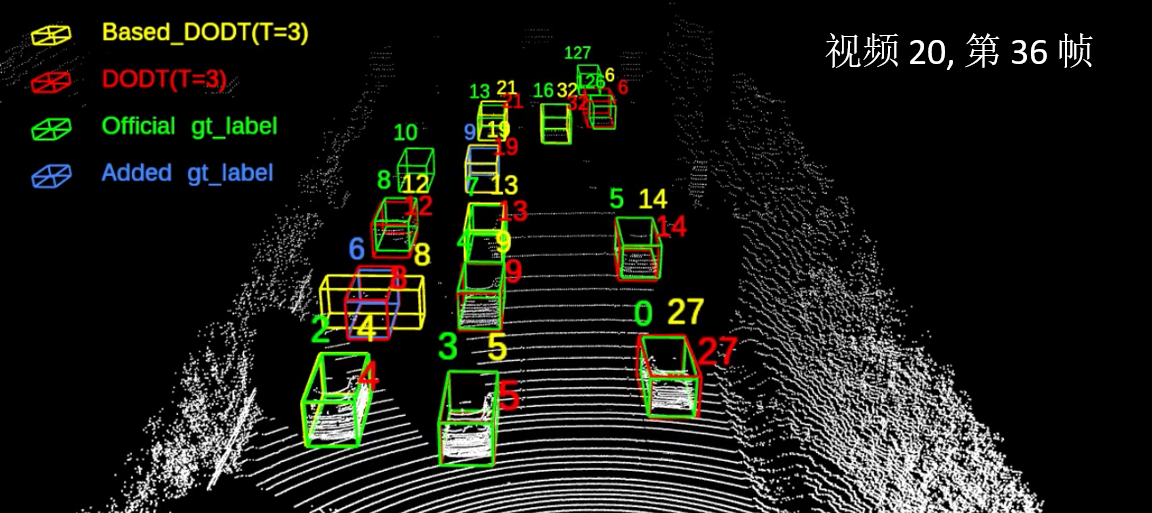
\includegraphics[width=\textwidth]{./imgs/viz_results/val/dodt_based_03.png}
	\caption{Based\_DODT与DODT($\tau=3$)对比结果。}
	\label{fig:dodt_based}
\end{figure}


\section{测试集结果展示}
\label{test_results}

本小节我们选择了KITTI目标追踪测试数据集中四段视频的连续四帧进行可视化。图\ref{fig:test_06}可视化的是第6段测试视频的连续四帧,场景为两辆车在公路上行驶;图\ref{fig:test_10}可视化的是第10段测试视频的连续四帧,是十字路口的车辆行驶场景;图\ref{fig:test_11}可视化的是第11段测试视频的连续四帧,场景是繁华的城市闹区;图\ref{fig:test_12}可视化的是第12段测试视频的连续四帧,场景中有较多停靠在路旁的车辆。所有图中每一行左侧为BEV视图,右侧上方为3D视图,右侧下方为图像视图,相同颜色表示同一辆车在不同时间的状态。

\begin{figure}
	\subfigure{
	\begin{minipage}[b]{0.4\linewidth}
		\begin{flushright}
			\begin{overpic}[scale=0.26]{./imgs/viz_results/06/bev/04.png}
				\put(5, 85){\color{red}{\small T = 3}}
			\end{overpic}\vspace{1pt}
			\begin{overpic}[scale=0.26]{./imgs/viz_results/06/bev/03.png}
				\put(5, 85){\color{red}{\small T = 2}}
			\end{overpic}\vspace{1pt}
			\begin{overpic}[scale=0.26]{./imgs/viz_results/06/bev/02.png}
				\put(5, 85){\color{red}{\small T = 1}}
			\end{overpic}\vspace{1pt}
			\begin{overpic}[scale=0.26]{./imgs/viz_results/06/bev/01.png}
				\put(5, 85){\color{red}{\small T = 0}}
			\end{overpic}
		\end{flushright}
	\end{minipage}}
	\subfigure{
	\begin{minipage}[b]{0.55\linewidth}
	\includegraphics[width=1\linewidth]{./imgs/viz_results/06/pc/04.png}\vspace{1pt}
	\includegraphics[width=1\linewidth]{./imgs/viz_results/06/img/04.png}\vspace{3.55pt}
	\includegraphics[width=1\linewidth]{./imgs/viz_results/06/pc/03.png}\vspace{1pt}
	\includegraphics[width=1\linewidth]{./imgs/viz_results/06/img/03.png}\vspace{3.55pt}
	\includegraphics[width=1\linewidth]{./imgs/viz_results/06/pc/02.png}\vspace{1pt}
	\includegraphics[width=1\linewidth]{./imgs/viz_results/06/img/02.png}\vspace{3.55pt}
	\includegraphics[width=1\linewidth]{./imgs/viz_results/06/pc/01.png}\vspace{1pt}
	\includegraphics[width=1\linewidth]{./imgs/viz_results/06/img/01.png}
	\end{minipage}}
	\caption{多目标追踪测试集视频片段6的连续四帧结果,场景为两辆车在公路上行驶。}
	\label{fig:test_06}
\end{figure}

\begin{figure}
	\centering
	\subfigure{
		\begin{minipage}[b]{0.45\linewidth}
			\begin{overpic}[scale=0.230]{./imgs/viz_results/10/bev/04.png}
				\put(5, 55){\color{red}{\small T = 3}}
			\end{overpic}\vspace{4pt}
			\begin{overpic}[scale=0.230]{./imgs/viz_results/10/bev/03.png}
				\put(5, 55){\color{red}{\small T = 2}}
			\end{overpic}\vspace{4pt}
			\begin{overpic}[scale=0.230]{./imgs/viz_results/10/bev/02.png}
				\put(5, 55){\color{red}{\small T = 1}}
			\end{overpic}\vspace{4pt}
			\begin{overpic}[scale=0.230]{./imgs/viz_results/10/bev/01.png}
				\put(5, 55){\color{red}{\small T = 0}}
			\end{overpic}
	\end{minipage}}
	\subfigure{
		\begin{minipage}[b]{0.47\linewidth}
			\includegraphics[width=1\linewidth]{./imgs/viz_results/10/pc/04.png}\vspace{1pt}
			\includegraphics[width=1\linewidth]{./imgs/viz_results/10/img/04.png}\vspace{2.5pt}
			\includegraphics[width=1\linewidth]{./imgs/viz_results/10/pc/03.png}\vspace{1pt}
			\includegraphics[width=1\linewidth]{./imgs/viz_results/10/img/03.png}\vspace{2.5pt}
			\includegraphics[width=1\linewidth]{./imgs/viz_results/10/pc/02.png}\vspace{1pt}
			\includegraphics[width=1\linewidth]{./imgs/viz_results/10/img/02.png}\vspace{2.5pt}
			\includegraphics[width=1\linewidth]{./imgs/viz_results/10/pc/01.png}\vspace{1pt}
			\includegraphics[width=1\linewidth]{./imgs/viz_results/10/img/01.png}
	\end{minipage}}
	\caption{多目标追踪测试集视频片段10的连续四帧结果,为十字路口的车辆行驶场景。}
	\label{fig:test_10}
\end{figure}

\begin{figure}
	%\centering
	\subfigure{
	\begin{minipage}[b]{0.4\linewidth}
	\begin{flushright}
		\begin{overpic}[trim={0cm, 3cm, 0cm, 0cm}, clip, scale=0.22]{./imgs/viz_results/11/bev/04.png}
			\put(5, 88){\color{red}{\small T = 3}}
		\end{overpic}\vspace{3pt}
		\begin{overpic}[trim={0cm, 3cm, 0cm, 0cm}, clip, scale=0.22]{./imgs/viz_results/11/bev/03.png}
			\put(5, 88){\color{red}{\small T = 2}}
		\end{overpic}\vspace{3pt}
		\begin{overpic}[trim={0cm, 3cm, 0cm, 0cm}, clip, scale=0.22]{./imgs/viz_results/11/bev/02.png}
			\put(5, 88){\color{red}{\small T = 1}}
		\end{overpic}\vspace{3pt}
		\begin{overpic}[trim={0cm, 3cm, 0cm, 0cm}, clip, scale=0.22]{./imgs/viz_results/11/bev/01.png}
			\put(5, 88){\color{red}{\small T = 0}}
		\end{overpic}
	\end{flushright}
	
	\end{minipage}}
	\subfigure{
	\begin{minipage}[b]{0.5\linewidth}
	\includegraphics[trim={0cm, 5.5cm, 0cm, 0cm}, clip,width=0.85\linewidth]{./imgs/viz_results/11/pc/04.png}\vspace{1pt}
	\includegraphics[width=0.85\linewidth]{./imgs/viz_results/11/img/04.png}\vspace{1.5pt}
	\includegraphics[trim={0cm, 5.5cm, 0cm, 0cm}, clip,width=0.85\linewidth]{./imgs/viz_results/11/pc/03.png}\vspace{1pt}
	\includegraphics[width=0.85\linewidth]{./imgs/viz_results/11/img/03.png}\vspace{1.5pt}
	\includegraphics[trim={0cm, 5.5cm, 0cm, 0cm}, clip,width=0.85\linewidth]{./imgs/viz_results/11/pc/02.png}\vspace{1pt}
	\includegraphics[width=0.85\linewidth]{./imgs/viz_results/11/img/02.png}\vspace{1.5pt}
	\includegraphics[trim={0cm, 5.5cm, 0cm, 0cm}, clip,width=0.85\linewidth]{./imgs/viz_results/11/pc/01.png}\vspace{1pt}
	\includegraphics[width=0.85\linewidth]{./imgs/viz_results/11/img/01.png}
	\end{minipage}}
	\caption{多目标追踪测试集视频片段11的连续四帧结果,场景是繁华的城市闹区。}
	\label{fig:test_11}
\end{figure}


\begin{figure}
	\centering
	\subfigure{
	\begin{minipage}[b]{0.42\linewidth}
	\begin{flushright}
		\begin{overpic}[scale=0.221]{./imgs/viz_results/12/bev/04.png}
			\put(5, 87){\color{red}{\small T = 3}}
		\end{overpic}\vspace{3pt}
		\begin{overpic}[scale=0.221]{./imgs/viz_results/12/bev/03.png}
			\put(5, 87){\color{red}{\small T = 2}}
		\end{overpic}\vspace{3pt}
		\begin{overpic}[scale=0.221]{./imgs/viz_results/12/bev/02.png}
			\put(5, 87){\color{red}{\small T = 1}}
		\end{overpic}\vspace{3pt}
		\begin{overpic}[scale=0.221]{./imgs/viz_results/12/bev/01.png}
			\put(5, 87){\color{red}{\small T = 0}}
		\end{overpic}
	\end{flushright}
	\end{minipage}}
	\subfigure{
	\begin{minipage}[b]{0.55\linewidth}
	\includegraphics[width=\linewidth]{./imgs/viz_results/12/pc/04.png}\vspace{1pt}
	\includegraphics[width=\linewidth]{./imgs/viz_results/12/img/04.png}\vspace{1.5pt}
	\includegraphics[width=\linewidth]{./imgs/viz_results/12/pc/03.png}\vspace{1pt}
	\includegraphics[width=\linewidth]{./imgs/viz_results/12/img/03.png}\vspace{1.5pt}
	\includegraphics[width=\linewidth]{./imgs/viz_results/12/pc/02.png}\vspace{1pt}
	\includegraphics[width=\linewidth]{./imgs/viz_results/12/img/02.png}\vspace{1.5pt}
	\includegraphics[width=\linewidth]{./imgs/viz_results/12/pc/01.png}\vspace{1pt}
	\includegraphics[width=\linewidth]{./imgs/viz_results/12/img/01.png}
	\end{minipage}}
	\caption{多目标追踪测试集视频片段12的连续四帧结果,有较多停靠在路旁的车辆。}
	\label{fig:test_12}
\end{figure}


% 打印时插入必要的空白页
\ifprint
	\newpage
	\thispagestyle{empty}
	\mbox{}
	
	% 避免空白页影响页码编号
	\clearpage
	\setcounter{page}{10}
\fi
